\section{Introduction}
The work presented in this thesis, being experimental in nature, hinges on numerous experimental techniques. The fundamental components of this work rely upon extensive use of X-ray diffraction (XRD) and transmission electron microscopy (TEM) in non-standard and novel ways. These techniques will be examined and examined in some detail, as their novel usage is integral to the work presented here. Several other experimental techniques are also utilized in this work, but they are used in their everyday implementations as seen in many papers in literature. These experimental techniques will be discussed only briefly for brevity. The two primary growth techniques used in this work will also be described, however as this work concentrates on epitaxy is a general phenomenon the intricacies and parameter spaces of these techniques will not be considered again for brevity.

\section{X-Ray}
X-rays are high energy photons, generated from the transitions of electrons between their core shell energy levels and bremsstrahlung (the acceleration of electrons). X-rays have a relatively weak interaction with matter, being absorbed or perturbed only slightly upon passing through it. X-rays have wavelengths comparable with the typical spacings between atoms in crystals, placing them as an ideal non-destructive probe for crystal structure. X-rays experience elastic scattering when interacting with the electrons surrounding atoms. The scattering of x-rays, combined with the 3D periodic structure of atoms, results in constructive and destructive interference and x-ray diffraction.
\begin{equation}
\label{eqn:bragg} 2d \sin(\theta) = n \lambda
\end{equation}
X-ray diffraction is fundamentally an interference phenomenon, for a set of planes within a crystal separated by some distance (d), they will diffract from those planes at an angle (\texttheta) depending upon the wavelength (\textlambda), this is known as Bragg's law as in \cref{eqn:bragg}. Bragg's law is identical to the phenomenon of thin film interference of visible light, only differing by the scale of the spacing and wavelengths. Bragg's law, while correct, is a one dimensional expression, in general it can be represented by the Laue Equations as in \cref{eqn:laue}. The vectors $k_i$ and $k_0$ are the incident and outgoing x-ray beam, $(a,b,c)$ is the primitive vector of the crystal lattice and $(h,k,l)$ are the reciprocal lattice indicies which must be integers. Thus, for a given crystal with a fixed unit cell, there are only certain relationships between the incident and outgoing x-ray beams that satisfy the diffraction conditions, resulting in diffraction.
\begin{align}
   a \cdot (k_0 - k_i) = 2 \pi h \\
   b \cdot (k_0 - k_i) = 2 \pi k \\
   c \cdot (k_0 - k_i) = 2 \pi l
   \label{eqn:laue}
\end{align}

A concept known as reciprocal, or momentum space, is a common construct used in solid state physics to disucss the properties of crystals. Reciprocal space can be visualized as a lattice of points, each representing a spacing present in the crystal, and the lattice having the same symmetry as the real crystal. Reciprocal space is also the Fourier partner of the real space lattice of the crystal. Reciprocal space provides an opportunity for an alternate expression of the conditions for diffraction, known as the Ewald construction. The Ewald construction or Ewald sphere expresses the diffraction condition through the overlay of a sphere of raidus 1/\textlambda{} pinned on its radius at the origin in reciprocal space, a incident X-ray beam ($k_i$) entering the sphere. The direction of the exiting diffraction beam is determined by the intersection of the surface of the sphere with the reciprocal lattice, as shown in \cref{fig:exp_xray_ewald}. As a crystal is rotated (or the incoming beam is moved), the ewald sphere will rotate about the origin, sweeping through reciprocal space and exciting diffraction conditions as the sphere coincides with lattice points. The pinned rotation of the Ewald sphere about the origin means that only reciprocal lattice points with a radius from the origin of less than 2/\textlambda{} can be excited into diffraction, indicating the effective limitation of a given x-ray source, as well as why light is an ineffective diffraction probe.
\begin{figure}
\centering
\missingfigure{Picture of ewald sphere construction from Bob He}
\caption{\label{fig:exp_xray_ewald}Ewald sphere construction of diffraction conditions}
\end{figure}


Stuff about intensity limitations (structure factor)

\subsection{2DXRD - Reciprocal Space Mapping}
\label{sec:2DXRD} As shown by \cref{eqn:laue} and \cref{fig:exp_xray_ewald}, there are an infinite number of orientations of a crystal which generate diffraction. For the purposes of the analysis of crystals, the lowest orders of crystal diffraction (small h,k,l) are the strongest, and provide the least ambiguous information. This still leaves a significant number of diffraction beams of interest to measure and provide structural information. The naive measurement technique for collecting this information involves taking a crystal and orienting an incoming x-ray beam, and a detector in configurations that satisfy \cref{eqn:laue}. Such measurements assume that the experimenter knows (or assumes) the orientation and unit cell of the crystal to a degree well enough calculate those configurations. If either of those pieces of information is unknown, the experimenter must instead sample the 4\textpi radians of angular space surrounding a crystal with sufficient resolution to collection the information they desire. Such experiments, when performed using a typical x-ray point detector, take inordinate amounts of time.
\begin{figure}
	\centering
	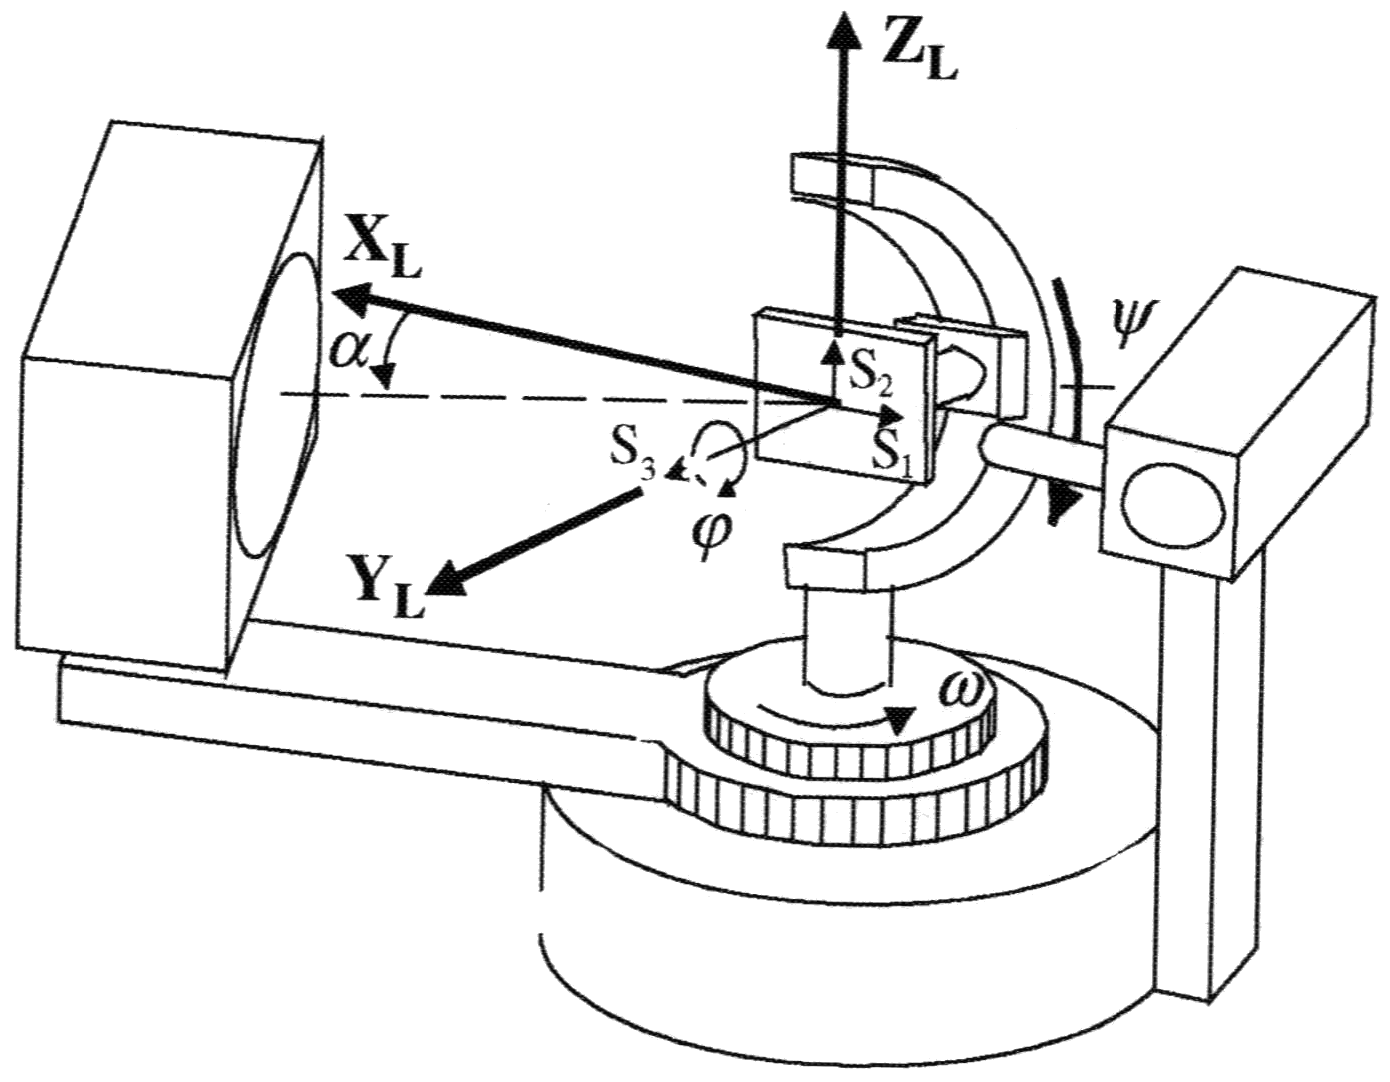
\includegraphics[width=0.9\textwidth]{exp_xray_machine}
    \caption{\label{fig:exp_xray_machine}Standard configuration of a 2DXRD system\cite{gadds_manual}}
\end{figure}
An alternate implementation of such a measurement process is through the use of a 2D planar detector rather than a point detector. A 2D x-ray detector can subtend a large section the angular space surrounding a given experiment, potentially collecting information about a large section of reciprocal space with each frame it collects as shown in \cref{fig:exp_xray_2dxrd}. If configuration is then swept through a range of diffraction conditions, the 2D detector will collect information about a wide swath of reciprocal space. 2DXRD techniques simultaneously collect information about the phase and symmetry of an unknown sample allowing that information to be then examined via a variety of techniques.
\begin{figure}
    \centering
    \missingfigure{diffraction to 2d detector from bob he}
    \caption{\label{fig:exp_xray_2dxrd}Intersection of diffraction with 2d x-ray detector}
\end{figure}


\subsection{High Resolution XRD}

\section{Electron Microscopy}
\section{TEM}
\section{STEM}
\section{SEM}

\section{Growth Techniques}
The work presented in this thesis are prepared primarily by two different growth methods, pulsed laser deposition (PLD) and molecular beam epitaxy (MBE). While these methods are quite distinct in their properties and the regimes under which they operate, the same material systems were not prepared by both systems, so direct comparisons cannot be made. Nevertheless, the differences between these growth processes will be examined in some detail to provide sufficient motivation for their choice for the given experiments.
\subsection{PLD}
\subsection{MBE}
\subsection{Thermal Dewetting}